\chapter{Background}\label{chap}

This chapter introduces the key concepts and theoretical foundations underpinning the thesis. It covers affect recognition in educational settings, deep-learning approaches for visual affect analysis, adaptive learning and reinforcement learning, and concludes with the stochastic modelling of temporal affective dynamics.

% ============================================================
\section{Emotion Recognition Formulation}\label{sec:bg:affect}
\paragraph{Affective sensing formulation.}
Let $x \in \mathcal{X}$ denote an observable input signal (e.g.\ a facial image or short video clip) captured during a learning activity. Emotion recognition is formulated as a supervised mapping problem $f:\mathcal{X} \rightarrow \mathcal{Y}$ that predicts a latent affective state $y \in \mathcal{Y}$ from $x$
\cite{lek_academic_2023,florestiyanto_emotion_2024}. When the input is restricted to facial imagery or video, the task is specifically referred to as \ac{FER} \cite{lek_academic_2023}.
% ============================================================
\section{Deep Learning Foundations}\label{sec:bg:dl}
% ============================================================
\subsection{Neural Networks and Supervised Learning}

A neural network is a type of machine learning model that learns to map inputs to outputs by passing data through multiple layers of transformations. Each layer applies a linear operation followed by a nonlinear activation function, enabling the model to learn increasingly complex patterns from the data \cite{goodfellow2016deep}.
The basic structure of a neural network is illustrated in Figure~\ref{fig:neural_network}.

\begin{figure}[h]
    \centering
    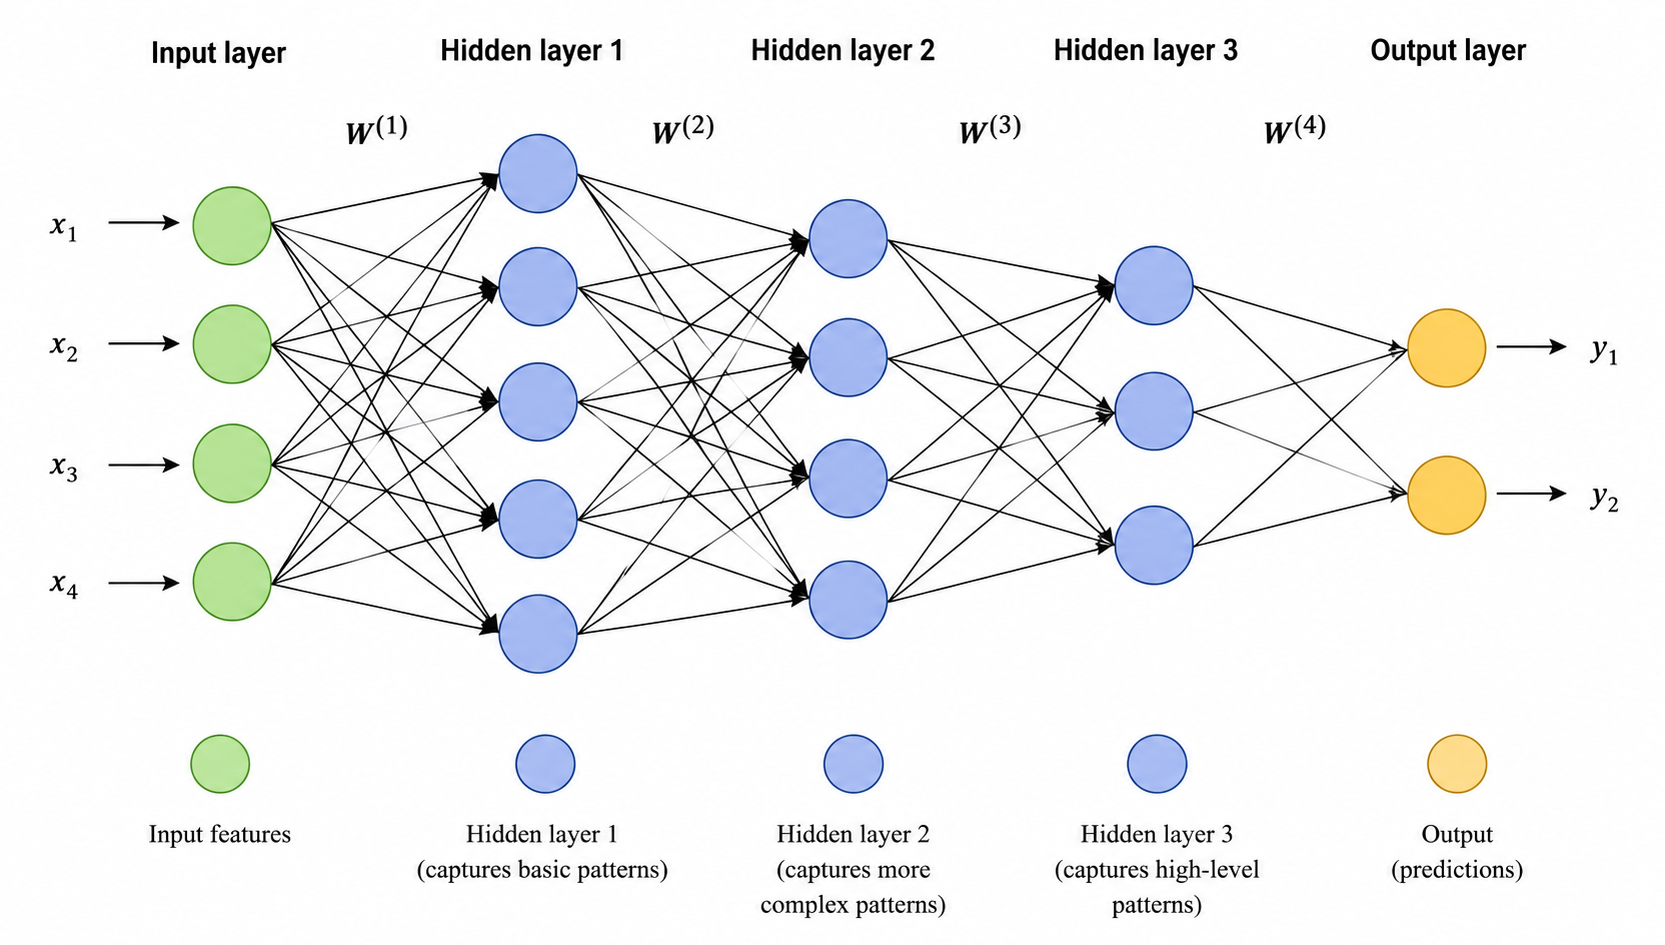
\includegraphics[width=0.7\textwidth]{Figures/neural network.png}
    \caption{Illustration of a basic neural network architecture with input, hidden, and output layers.}
    \label{fig:neural_network}
\end{figure}

In supervised learning, the model is trained using labeled examples $(x_i, y_i)$, where each input is paired with a corresponding target output. The objective is to learn model parameters that minimize a loss function over the training dataset. This optimization is commonly performed using stochastic gradient descent.

Deep learning refers to neural networks with multiple hidden layers. The presence of depth enables hierarchical representation learning, where earlier layers capture low-level features and deeper layers encode more abstract and task-specific representations \cite{goodfellow2016deep}.

\subsection{Activation Functions}\label{sec:bg:activations}
% ------------------------------------------------------------

Activation functions introduce nonlinearity into neural networks, allowing 
them to learn complex patterns beyond linear mappings. The most commonly 
used activation functions in this thesis are \cite{siswantoro_facial_2024}:

\begin{align}
\text{ReLU:}&\quad \sigma(z) = \max(0, z), \\
\text{Sigmoid:}&\quad \sigma(z) = \frac{1}{1+e^{-z}}, \\
\text{Tanh:}&\quad \sigma(z) = \frac{e^z - e^{-z}}{e^z + e^{-z}}, \\
\text{Softmax:}&\quad \sigma(\mathbf{z})_i =
\frac{e^{z_i}}{\sum_j e^{z_j}}.
\end{align}

ReLU is the standard activation for hidden layers due to its simplicity 
and efficiency \cite{siswantoro_facial_2024}. Sigmoid is typically used 
for binary or multi-label outputs \cite{siswantoro_facial_2024}. Tanh is 
commonly used in recurrent networks due to its zero-centered output 
\cite{siswantoro_facial_2024}. Softmax is used in multi-class 
classification to produce a probability distribution over classes 
\cite{siswantoro_facial_2024}.

ReLU outputs zero for all negative inputs and grows linearly for positive 
ones, making it fast to train and free of the vanishing gradient problem 
that affects bounded activations \cite{siswantoro_facial_2024}. Sigmoid 
squashes any input to the range $(0, 1)$, which makes it suitable for 
independent binary predictions but susceptible to vanishing gradients at 
saturation \cite{siswantoro_facial_2024}. Tanh maps inputs to $(-1, 1)$ 
and is zero-centred, which reduces the gradient update bias present in 
sigmoid and makes it the standard choice for recurrent hidden states 
\cite{siswantoro_facial_2024}. Softmax normalises a vector of scores into 
a probability distribution summing to one, making it appropriate for 
mutually exclusive multi-class outputs rather than the independent binary 
predictions of sigmoid \cite{siswantoro_facial_2024}.

\subsection{Convolutional Neural Networks}\label{sec:bg:cnn}

% ------------------------------------------------------------

A \ac{CNN} is a type of neural network designed for image data. Instead of using fully connected layers, \ac{CNN}s apply convolution operations that slide small filters (kernels) over the input image to extract features such as edges, textures, and shapes.

Mathematically, a convolution layer computes feature maps by applying learned kernels across local regions of the input image, producing outputs that preserve spatial structure \cite{aly_revolutionizing_2025}.

\ac{CNN}s are widely used in computer vision because they rely on three key ideas: local connectivity (each neuron sees only a small region), weight sharing (the same filter is reused across the image), and translation equivariance, meaning that shifting the input leads to a corresponding shift in the output \cite{aly_revolutionizing_2025,gupta_edfa_2023}.

A \ac{CNN} is usually used as a feature extractor (backbone), where the network converts an image into a compact representation before classification. When pretrained on large datasets such as ImageNet, these models can be reused for new tasks through transfer learning, where the learned features are adapted to a smaller dataset \cite{komaravalli_detecting_2023,aly_revolutionizing_2025}.
The convolutional neural network pipeline used for feature extraction is shown in Figure~\ref{fig:cnn_simple}.

\begin{figure}[h]
    \centering
    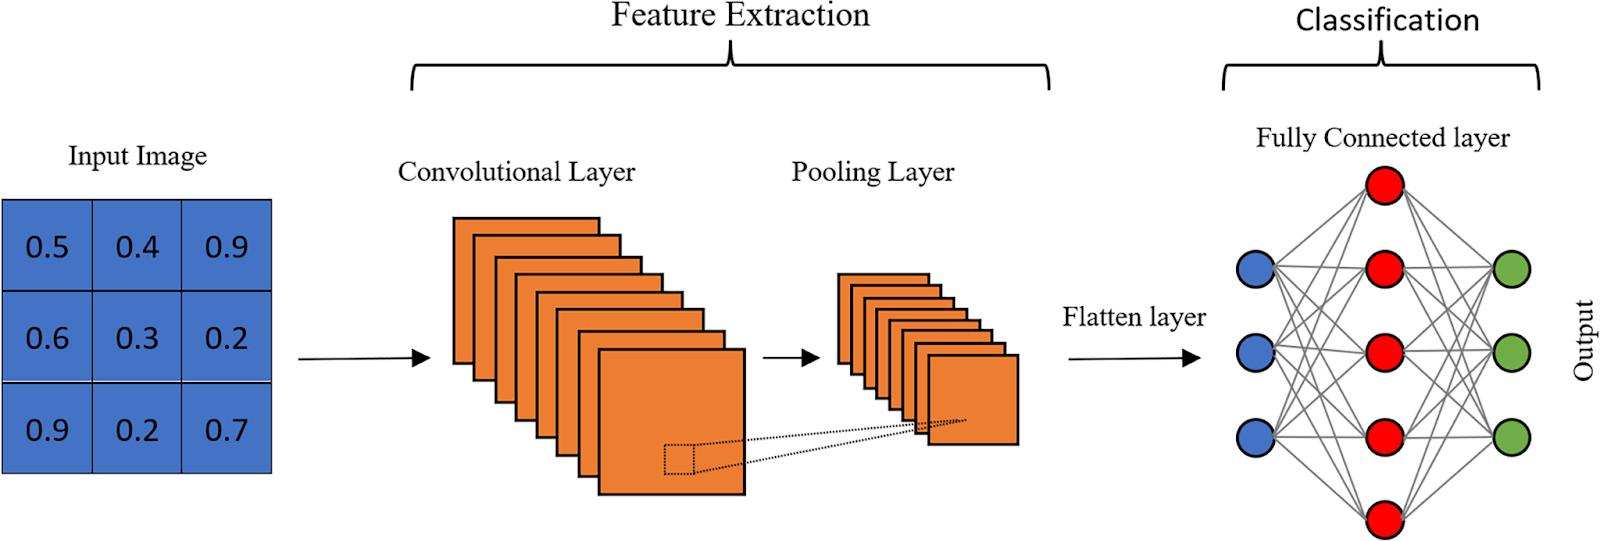
\includegraphics[width=0.85\textwidth]{Figures/cnn.png}


\caption{Basic architecture of a Convolutional Neural Network showing convolution, pooling, and classification stages. Adapted from \cite{alsaleh2023efficientcnn}.}
    \label{fig:cnn_simple}
\end{figure}

% ------------------------------------------------------------
\subsection{Residual Learning and Major \ac{CNN} Backbone Families}
\label{sec:bg:residual}

As convolutional neural networks become deeper, they can become more difficult to train. Adding additional layers does not always improve performance because gradients may become weaker as they propagate through the network \cite{he_resnet_2016}.This issue is known as the degradation problem .

To address this challenge,\cite{he_resnet_2016} introduced residual learning in the ResNet architecture. Instead of learning the desired mapping directly, each block learns a residual function that is added to the original input through a skip connection. 

\paragraph{ResNet \cite{he_resnet_2016}.}
\ac{ResNet} is a widely used \ac{CNN} architecture that introduces skip connections between layers. These connections allow information and gradients to flow more easily through the network, making it possible to train much deeper models than traditional \ac{CNN}s .

Several versions of ResNet have been proposed, including ResNet-18, ResNet-34, ResNet-50, ResNet-101, and ResNet-152, which differ mainly in network depth. Among them, ResNet-50 is one of the most popular models because it provides a good balance between accuracy and computational cost. Due to its strong feature extraction capabilities and availability of pretrained weights, ResNet-50 is widely used as a backbone network in facial expression recognition and other computer vision tasks \cite{he_resnet_2016}.


\paragraph{EfficientNet \cite{tan_efficientnet_2019,tan_efficientnetv2_2021}.}
EfficientNet is a family of convolutional neural networks designed to achieve high accuracy while using fewer parameters and computational resources than many traditional \ac{CNN}s. The architecture scales network depth, width, and input resolution in a balanced manner, allowing larger models to improve performance efficiently. EfficientNetV2 further improves training speed and computational efficiency while maintaining strong accuracy. Due to these advantages, EfficientNet models are widely used in computer vision tasks, including facial expression recognition \cite{tan_efficientnet_2019,tan_efficientnetv2_2021}.

\paragraph{ShuffleNetV2 \cite{ma_shufflenetv2_2018}.}
ShuffleNetV2 is a lightweight \ac{CNN} architecture designed for fast and efficient inference on devices with limited computational resources. It reduces computational cost while maintaining competitive accuracy through an efficient network design. As a result, ShuffleNetV2 is commonly used in real-time and mobile vision applications where speed and efficiency are important \cite{ma_shufflenetv2_2018}.
% ------------------------------------------------------------
\subsection{Recurrent Neural Networks and \ac{LSTM}}\label{sec:bg:rnn}
% ------------------------------------------------------------

Recurrent Neural Networks (RNNs) are designed to process sequential data such as time series or text. Unlike feedforward networks, RNNs maintain a hidden state that is updated at each time step, allowing the model to capture temporal dependencies in a sequence \cite{hochreiter_lstm_1997}.

However, standard RNNs struggle to learn long-term dependencies due to vanishing and exploding gradients, which makes training unstable on long sequences \cite{hochreiter_lstm_1997}.

To address this issue, \ac{LSTM} networks were introduced. \ac{LSTM}s improve RNNs by adding a memory cell that can store information over long time periods. This memory is controlled by gates that decide what information to keep, forget, or output, allowing the model to selectively retain important information while discarding irrelevant details \cite{hochreiter_lstm_1997}.

A \ac{BiLSTM} further improves this idea by processing the sequence in both forward and backward directions. This allows the model to use both past and future context when representing each time step \cite{leong_deep_2020,asaju_adaptive_2022}.
The \ac{BiLSTM} architecture, illustrating the forward and backward state processing across time steps, is shown in Figure~\ref{fig:cnn_bilstm}.

\begin{figure}[h]
    \centering
    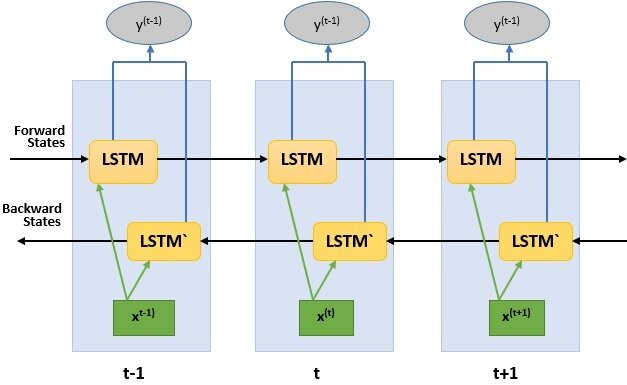
\includegraphics[width=0.85\textwidth]{Figures/bilstm.png}
  \caption{Bidirectional \ac{LSTM} architecture showing forward and backward hidden state propagation across time steps (adapted from \cite{elsayed2021cnnbilstm}).}
    \label{fig:cnn_bilstm}
\end{figure}
% ------------------------------------------------------------
\subsection{Training Regularisation and Stability}
\label{sec:bg:regularisation}
% ------------------------------------------------------------

\paragraph{Dropout \cite{srivastava_dropout_2014}.}
Dropout is a technique used to reduce overfitting in neural networks. During training, it randomly disables some neurons so the model does not rely too much on specific features. During inference, all neurons are used with scaled outputs to maintain consistency \cite{srivastava_dropout_2014}.

\paragraph{Batch Normalisation \cite{ioffe_bn_2015}.}
Batch Normalisation improves training stability by normalising layer inputs. This helps the network train faster, reduces sensitivity to initialization, and allows higher learning rates \cite{ioffe_bn_2015}.

\paragraph{Gradient Clipping.}
Gradient clipping prevents unstable training by limiting very large gradients during backpropagation. This is especially useful in recurrent models, where gradients can explode over long sequences.
\subsection{Adaptive Gradient Optimisers: Adam and AdamW}
\label{sec:bg:adam}
% ------------------------------------------------------------

Adam is an adaptive optimisation algorithm that adjusts the learning rate for each parameter using running averages of past gradients \cite{kingma_adam_2015}. This makes training faster and more stable compared to standard SGD.

AdamW improves Adam by separating weight decay from the gradient update. This leads to more effective regularisation and better generalisation performance \cite{loshchilov_adamw_2019}.
% ------------------------------------------------------------
\subsection{Supporting Architectures and Classical Methods}
\label{sec:bg:glossary}
% ------------------------------------------------------------

\paragraph{DenseNet \cite{huang_densenet_2017}.}
DenseNet connects each layer to all later layers, improving feature reuse and gradient flow while using fewer parameters.

\paragraph{3D DenseNet \cite{mehta_three-dimensional_2022}.}
3D DenseNet extends DenseNet to video data using 3D convolutions for spatial-temporal learning.

\paragraph{Xception \cite{chollet_xception_2017}.}
Xception uses depthwise separable convolutions to reduce computation while keeping strong feature extraction ability.

\paragraph{VGG-19 \cite{simonyan_vgg_2015}.}
VGG-19 is a simple deep \ac{CNN} made of stacked $3\times3$ convolutions. It is mainly used as an early transfer learning backbone.

\paragraph{\ac{GRU} and Bi-\ac{GRU} \cite{cho_gru_2014}.}
\ac{GRU} is a simpler version of \ac{LSTM} with fewer gates. Bi-\ac{GRU} processes sequences in both directions to capture past and future context.

\paragraph{C3D \cite{tran_c3d_2015}.}
C3D uses 3D convolutions to learn spatial and temporal features directly from video clips.

\paragraph{LRCN \cite{donahue_lrcn_2015}.}
LRCN combines \ac{CNN}s for frame feature extraction and \ac{LSTM}s for modeling temporal sequences.

\paragraph{\ac{TCN} \cite{bai_tcn_2018}.}
\ac{TCN} replaces recurrent networks with dilated convolutions for efficient sequence modeling.

\paragraph{CBAM \cite{woo_cbam_2018}.}
CBAM is an attention module that improves \ac{CNN} features by focusing on important channels and spatial regions.

\paragraph{\ac{HOG} \cite{dalal_hog_2005}.}
\ac{HOG} is a hand-crafted feature descriptor based on image gradients, used in classical vision tasks.

\paragraph{\ac{LBP} \cite{ojala_lbp_2002}.}
\ac{LBP} describes local texture patterns by comparing pixel intensities with neighbors.

\paragraph{\ac{SVM} \cite{cortes_svm_1995}.}
\ac{SVM} is a classical classifier that finds a decision boundary with maximum margin, often used with \ac{HOG} or \ac{LBP} features.

% ============================================================
\section{Video Representation Learning}\label{sec:bg:video}
% ============================================================

A video is a sequence of frames represented as a tensor. Unlike images, video data contains both spatial information (what appears in each frame) and temporal information (how content changes over time) \cite{asaju_adaptive_2022,mehta_three-dimensional_2022,abedi_improving_2021}.

\paragraph{Frame sampling.}
Processing all frames in a video is usually unnecessary and computationally expensive. Therefore, a fixed number of frames is selected from each video. This reduces redundancy and makes training more efficient, but may also lose some temporal details \cite{abedi_improving_2021,asaju_adaptive_2022}.

\paragraph{Spatio-temporal model approaches.}
There are three common ways to model video data:

\begin{enumerate}
  \item \textbf{\ac{CNN} + RNN:} A \ac{CNN} extracts features from each frame, and an \ac{LSTM} or \ac{BiLSTM} processes the sequence over time.
  \item \textbf{3D \ac{CNN}:} A single model learns both spatial and temporal features directly using 3D convolutions.
  \item \textbf{Transformer-based models:} Frames are treated as tokens and related using self-attention to capture temporal dependencies.
\end{enumerate}

These approaches are different ways of combining spatial and temporal information, and the choice depends on the application and computational constraints.

% ============================================================
\section{Attention Mechanisms}\label{sec:bg:attention}
% ============================================================

Attention mechanisms allow a model to focus on the most relevant parts of an input instead of treating all features equally. They assign different importance weights to different elements and combine them into a weighted representation \cite{vaswani_attention_2017}.

% ------------------------------------------------------------
\subsection{Self-Attention and Multi-Head Attention}
\label{sec:bg:selfattn}
% ------------------------------------------------------------

Self-attention is a mechanism where each element in a sequence compares itself with all other elements to determine which parts are most relevant. This allows the model to capture long-range dependencies more effectively than traditional sequential models \cite{vaswani_attention_2017}.

In self-attention, each input element is transformed into queries, keys, and values. The similarity between queries and keys is used to compute attention weights, which are then applied to the values to produce the final output \cite{vaswani_attention_2017}.

\paragraph{Multi-head attention \cite{vaswani_attention_2017}.}
Multi-head attention improves self-attention by using multiple attention “heads” in parallel. Each head learns different relationships in the data, and the results are combined to form a richer representation.

A Transformer layer is built by stacking multi-head attention with a feed-forward network and residual connections. This architecture allows efficient modeling of relationships across entire sequences \cite{vaswani_attention_2017}. Vision Transformers extend this idea to images by treating image patches as sequence tokens \cite{su_leveraging_2024}.

\subsection{Channel and Spatial Attention}\label{sec:bg:channel_spatial}
% ------------------------------------------------------------

For a \ac{CNN} feature map $F \in \mathbb{R}^{H \times W \times C}$, attention can be applied in different ways to improve feature representation.

\paragraph{Channel attention.}
Channel attention learns the importance of each feature channel and reweights them accordingly. The \ac{SE} block is a common approach, where global information from each channel is first aggregated and then passed through a small neural network to generate channel-wise importance scores. These scores are used to rescale the feature channels, allowing the model to focus on the most useful features \cite{hu_squeeze_2018}.

\paragraph{Spatial attention.}
Spatial attention focuses on \textit{where} important information appears in the feature map. It learns a spatial mask that highlights informative regions while suppressing less relevant areas, improving the model’s ability to localise important visual cues \cite{aly_revolutionizing_2025}.

\subsection{Temporal Attention}\label{sec:bg:tempattn}
% ------------------------------------------------------------

Temporal attention is used to model how important different frames are in a video. Instead of treating all frames equally, it assigns higher weights to more informative frames.

The final video representation is computed as a weighted combination of frame features, where the weights reflect the importance of each frame. This allows the model to focus on key moments where emotional or semantic information is more evident \cite{mehta_three-dimensional_2022,su_leveraging_2024}.

Temporal attention is especially useful when relevant information appears only in a few frames rather than uniformly across the entire video.


% ============================================================
\section{Intelligent Tutoring Systems and Knowledge Tracing}
\label{sec:bg:its}
% ============================================================

\subsection{Intelligent Tutoring Systems}

An \ac{ITS} is an AI-based learning system that adapts instruction to each learner. It typically considers three main parts: the learner model (student state), the domain model (learning content), and the pedagogical model (how the system teaches) \cite{zerkouk_comprehensive_2025,kabudi_ai-enabled_2021}.

By continuously observing the learner and updating its internal state, an \ac{ITS} can adjust feedback, difficulty, and learning content in a dynamic way.

% ------------------------------------------------------------

\subsection{Knowledge Tracing}\label{sec:bg:kt}

\ac{KT} refers to the task of estimating a learner’s knowledge over time based on their past interactions \cite{urbaite_adaptive_2026,kuling_ken_2025}. It uses sequences of student responses to predict future performance and track learning progress.

Traditional approaches model knowledge as a hidden state that evolves over time, while modern deep learning approaches use recurrent neural networks to learn this progression directly from data (Deep Knowledge Tracing).

\ac{KT} focuses on predicting student performance, but does not decide what action to take next. That role is handled by a separate decision-making module in intelligent tutoring systems.

\section{Reinforcement Learning}\label{sec:bg:rl}
% ============================================================

\ac{RL} is a framework for sequential decision-making, where an agent learns to choose actions based on feedback from the environment \cite{sutton_rl_book_2018}. The goal is to learn a policy that maximises long-term reward through trial and error interaction.
\subsection{Markov Decision Processes}\label{sec:bg:mdp}
% ------------------------------------------------------------

A \ac{MDP} is a framework used to model sequential decision-making problems. It consists of states $\mathcal{S}$, actions $\mathcal{A}$, a transition function $P$, a reward function $R$, and a discount factor $\gamma$ \cite{sutton_rl_book_2018}.

The key assumption is the \emph{Markov property}, which states that the next state depends only on the current state and action, not on past history.

A policy $\pi$ defines how an agent selects actions based on the current state. The goal of reinforcement learning is to learn a policy that maximises the expected long-term reward.

In simple terms, an \ac{MDP} describes how an agent interacts with an environment step by step in order to maximise cumulative reward.

\subsection{Partially Observable Markov Decision Processes}
\label{sec:bg:pomdp}
% ------------------------------------------------------------

In many real-world problems, the agent cannot directly observe the full environment state. Instead, it receives partial or noisy observations. This setting is modeled using a \ac{POMDP} \cite{kaelbling_pomdp_1998}.

A \ac{POMDP} extends an \ac{MDP} by introducing observations, meaning the agent must make decisions based on incomplete information.

Since the true state is not fully visible, the agent relies on past observations or an internal memory to estimate the current situation.

In practice, deep reinforcement learning models handle this limitation using recurrent networks or by summarising recent observations.
\subsection{Model-Based vs.\ Model-Free Reinforcement Learning}
% ------------------------------------------------------------

Reinforcement learning methods are generally divided into two categories: model-based and model-free approaches.

Model-based methods use an explicit model of the environment to predict how states change and to plan future actions. In contrast, model-free methods learn directly from experience without modeling the environment dynamics \cite{sutton_rl_book_2018}.

Model-free approaches are more commonly used in complex real-world problems where building an accurate environment model is difficult or impractical.

\subsection{Exploration and Exploitation}
% ------------------------------------------------------------

A key challenge in reinforcement learning is balancing exploration and exploitation.

\emph{Exploration} means trying new actions to discover better strategies, while \emph{exploitation} means choosing the best-known action based on current knowledge \cite{sutton_rl_book_2018}.

A common strategy is the $\varepsilon$-greedy policy, where the agent mostly chooses the best-known action but occasionally selects a random action to explore the environment.
\subsection{Q-Learning}\label{sec:bg:qlearning}
% ------------------------------------------------------------

Q-learning is a reinforcement learning method that learns how good an action is in a given state without requiring a model of the environment \cite{sutton_rl_book_2018}.

It learns a function $Q(s,a)$ that estimates the long-term reward of taking action $a$ in state $s$. The update rule improves this estimate using the reward received and the best estimated future action.

Q-learning is called \emph{off-policy} because it learns from the best possible action rather than the action actually taken. It works well in small, discrete environments but does not scale to high-dimensional problems.
The mapping from state representations to action-value outputs in Q-learning is illustrated in Figure~\ref{fig:q_values}.
\begin{figure}[h]
    \centering
    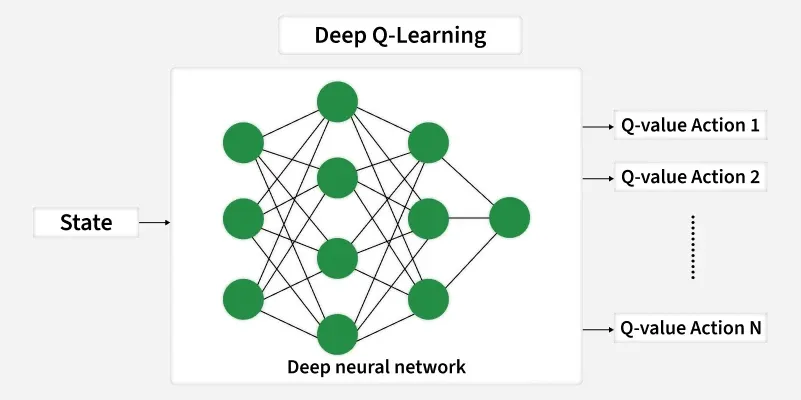
\includegraphics[width=0.6\textwidth]{Figures/deep.png}
    \caption{Mapping from input state to action-value outputs $Q(s,a)$, where each action receives a separate Q-score used for decision making.}
    \label{fig:q_values}
\end{figure}

\subsection{Deep Q-Networks}\label{sec:bg:dqn}
% ------------------------------------------------------------

\ac{DQN} extend Q-learning by using a neural network to approximate the Q-function instead of a table \cite{mnih_dqn_2015}. This allows the method to handle high-dimensional inputs such as images.

Two key ideas make \ac{DQN} stable:

\begin{itemize}
  \item \textbf{Experience replay:} past experiences are stored and randomly sampled during training to reduce correlation between updates.
  \item \textbf{Target network:} a separate, slowly updated network is used to compute learning targets, which stabilises training.
\end{itemize}

\ac{DQN} is designed for discrete action spaces, where the best action is selected by comparing all possible actions.
\section{Simulation-Based Evaluation in Reinforcement Learning}\label{sec:bg:simulation}

The reinforcement learning interaction loop between agent and environment is shown in Figure~\ref{fig:rl_sequence}.

\begin{figure}[h]
    \centering
    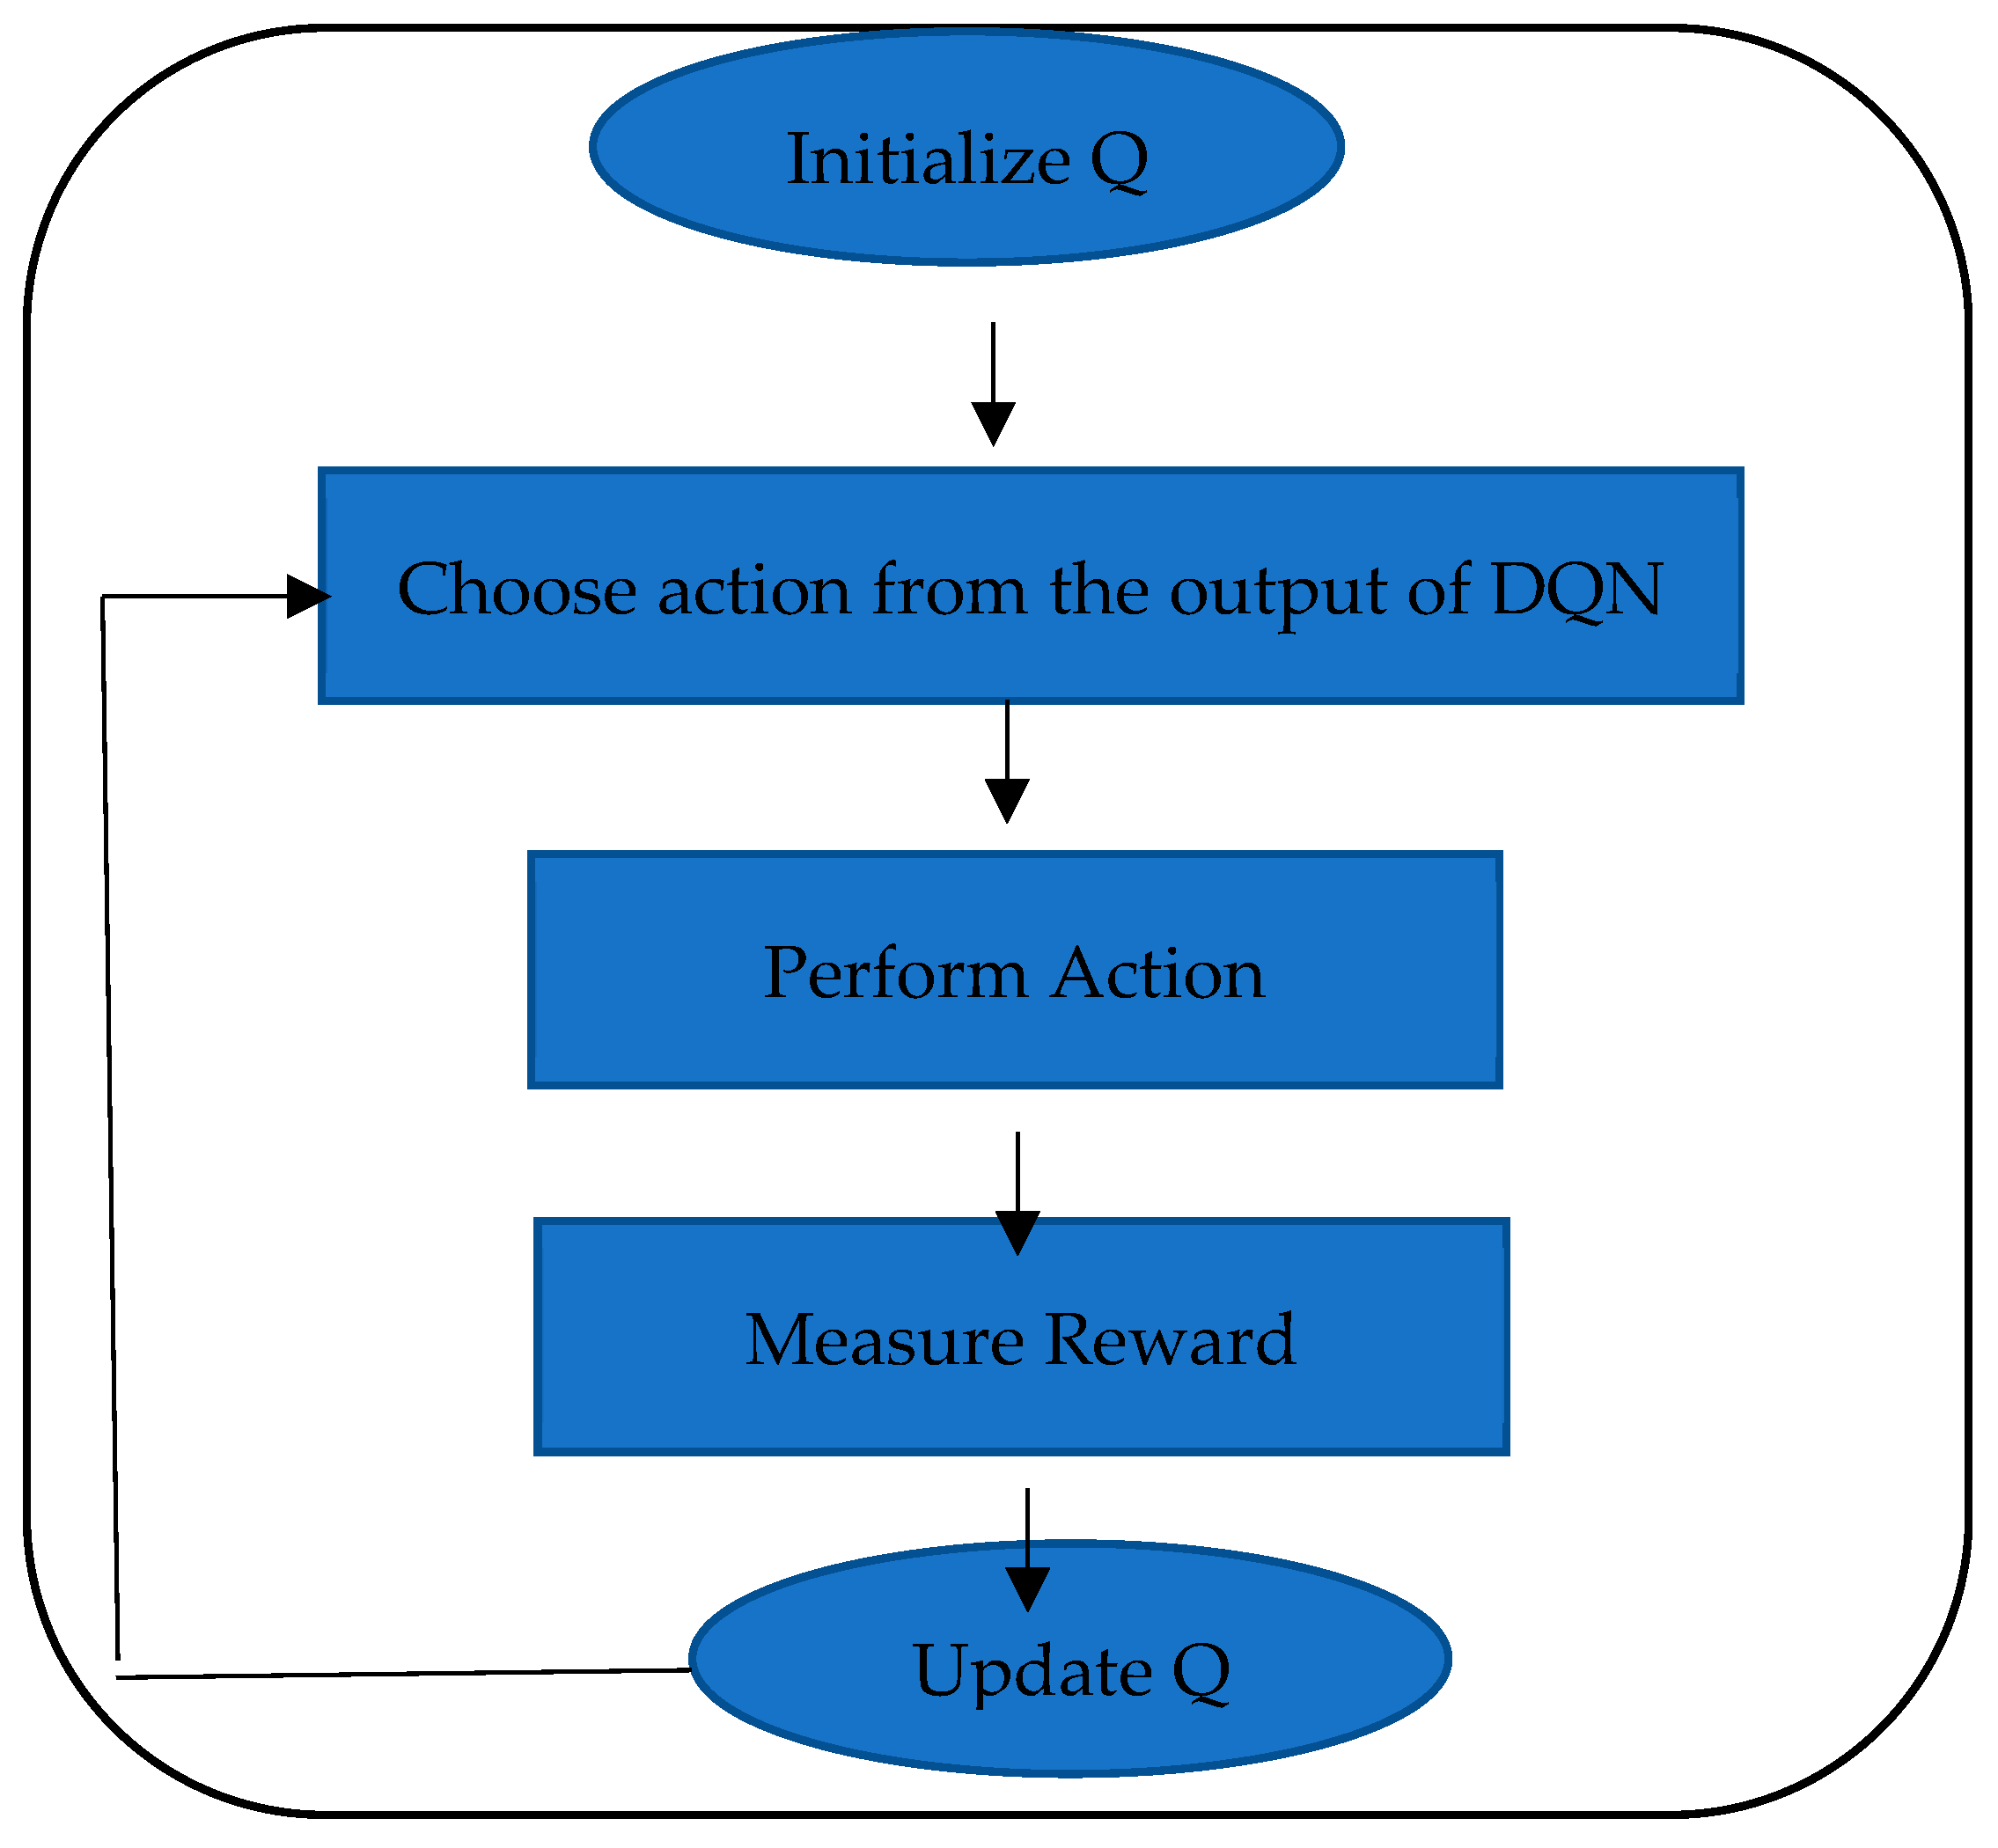
\includegraphics[width=0.45\textwidth]{Figures/Initialize Q.png}
    \caption{Reinforcement learning interaction loop showing the sequence of state observation, action selection, reward feedback, and environment transition.}
    \label{fig:rl_sequence}
\end{figure}

% ============================================================

Reinforcement learning methods are typically trained and evaluated in simulated environments due to the large number of interactions required for learning \cite{sutton_rl_book_2018}.

Simulation allows safe and scalable training before deploying models in real-world or human-centered systems such as intelligent tutoring systems.

However, results obtained in simulation may not fully transfer to real environments due to differences between the simulated and real dynamics, known as the sim-to-real gap \cite{azoulay_adaptive_2021}.

Therefore, simulation results are best interpreted as controlled approximations of real-world behaviour.

The complete Deep Q-Network training pipeline, including experience replay and target network updates, is shown in Figure~\ref{fig:dqn_pipeline}.

\begin{figure}[h]
    \centering
    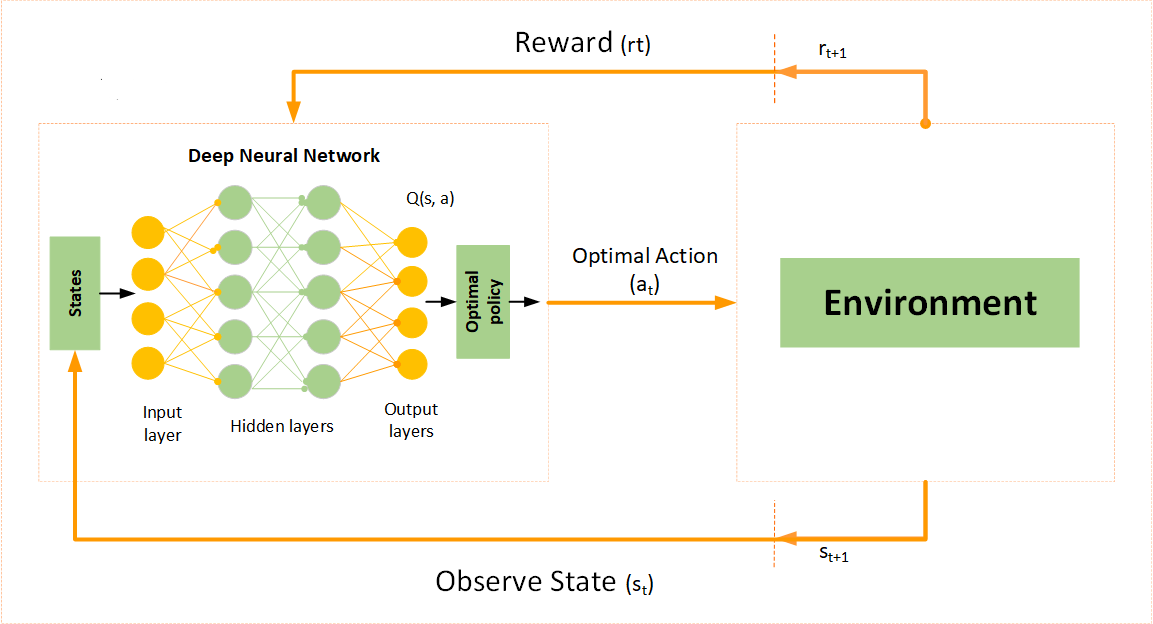
\includegraphics[width=0.6\textwidth]{Figures/full.png}
    \caption{\ac{DQN} training cycle including experience replay, target network updates, and Q-value optimization.}
    \label{fig:dqn_pipeline}
\end{figure}
